\section{Реализация}

\subsection{Суть и назначение агента}

За время обучения студенты направления <<Математика и компьютерные науки>>
СПбПУ сталкнулись с трудностями при чтении и понимании презентаций в PDF формате, в которых
материал изложен неструктурированно, содержит большое
количество примеров, которые на первый взгляд не относятся к теме, а также множество
визуального шума. В результате чтение таких презентаций не вдохновляет на учёбу,
а скорее утомляет и затрудняет усвоение материала.

Разработанный ИИ-агент <<Study Agent>> --- это приложение с веб-интерфейсом,
которое получает на вход PDF-презентации и преобразует их
в структурированный интерактивный конспект для изучения материала.

Агент решает задачу самостоятельного изучения материала, изложенного в презентациях,
избавляя студента от утомительной работы с неструктурированным исходным текстом.

Взаимодействие студента с агентом устроено последовательно.

Сначала студент загружает одну или несколько презентаций в систему.
Агент извлекает из них текст, анализирует его и выделяет список тем,
изложенных в презентациях.

Полученный список тем предъявляется студенту для подтверждения
(hitl), на этом этапе можно удалять уже выделенные темы или добавлять свои,
после подтверждения запускается генерация карточек.

Карточка составляется для каждой темы и содердит:
\begin{itemize}
    \item исходный текст из презентации по данной теме;
    \item этот же текст, переформулированный более простым языком;
    \item примеры из интернета, похожие на примеры из презентации.
\end{itemize}
Кроме того, агент сообщает о наличии или отсутствии ошибок в презентации
с пояснением, в чём именно состоит ошибка.

При изучении готовых карточек студент может задавать вопросы в чате
с ИИ, который отвечает с опорой на материалы конкретной темы.

\subsection{Архитектура и алгоритм работы}

Приложение построено по клиент-серверной архитектуре: бэкенд на Python (FastAPI)
с базой данных SQLite обслуживает веб-интерфейс, а прогресс обработки передаётся
в браузер в реальном времени. Логика агента описана в виде графа состояний
в библиотеке LangGraph, запросы к языковой модели выполняются через
OpenAI-совместимый API (по умолчанию --- DeepSeek), текст из PDF извлекается
библиотекой PyMuPDF с распознаванием текста на изображениях через OCR
(Tesseract), примеры подбираются веб-поиском DuckDuckGo. Приложение упаковано
в Docker-контейнер и запускается через docker-compose. Граф агента состоит
из трёх последовательных узлов:
\begin{enumerate}
    \item \textit{Извлечение тем} --- модель выделяет темы из текста
          презентаций, дубликаты объединяются.
    \item \textit{Подтверждение тем} --- граф ждёт, пока пользователь проверит
          и подтвердит список.
    \item \textit{Генерация карточек} --- по каждой теме модель собирает
          конспект, проверяет его на ошибки, упрощает и ищет примеры в интернете.
\end{enumerate}

Агент конечен. Граф ---
это линейная цепочка из трёх узлов, завершающаяся узлом END. Все повторения
внутри узлов ограничены: рекурсия деления фрагментов --- не глубже
пяти уровней, слияние тем --- до двенадцати в списке, генерация карточек ---
один проход по конечному списку тем.

\subsection{Результаты работы}

Работа агента была проверена на лекционных презентациях курса; ниже показаны
основные этапы в интерфейсе.

На рисунке~\ref{fig:upload} показан начальный экран, где пользователь
загружает одну или несколько PDF-презентаций и запускает извлечение тем.
\begin{figure}[H]
    \centering
    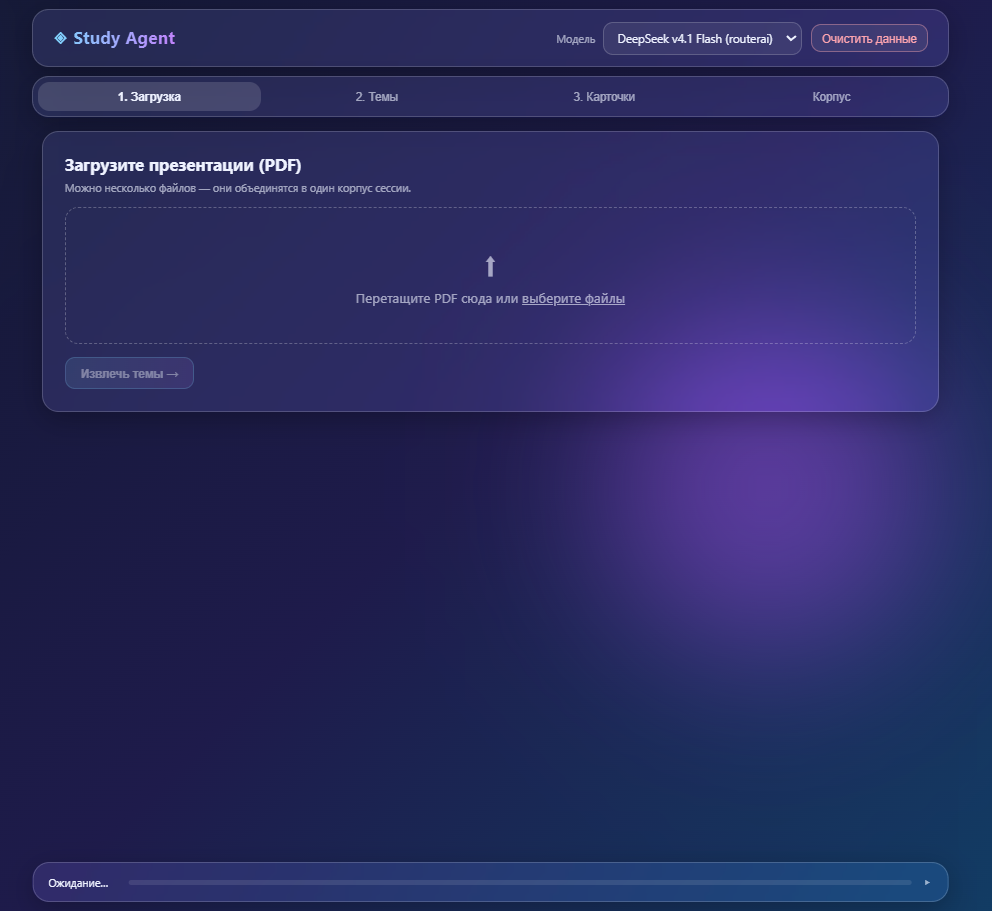
\includegraphics[width=0.85\textwidth]{images/загрузка_файла.png}
    \caption{Этап загрузки презентаций}
    \label{fig:upload}
\end{figure}

После анализа корпуса агент выводит список извлечённых тем, который пользователь
может отредактировать и подтвердить (рис.~\ref{fig:topics}).
\begin{figure}[H]
    \centering
    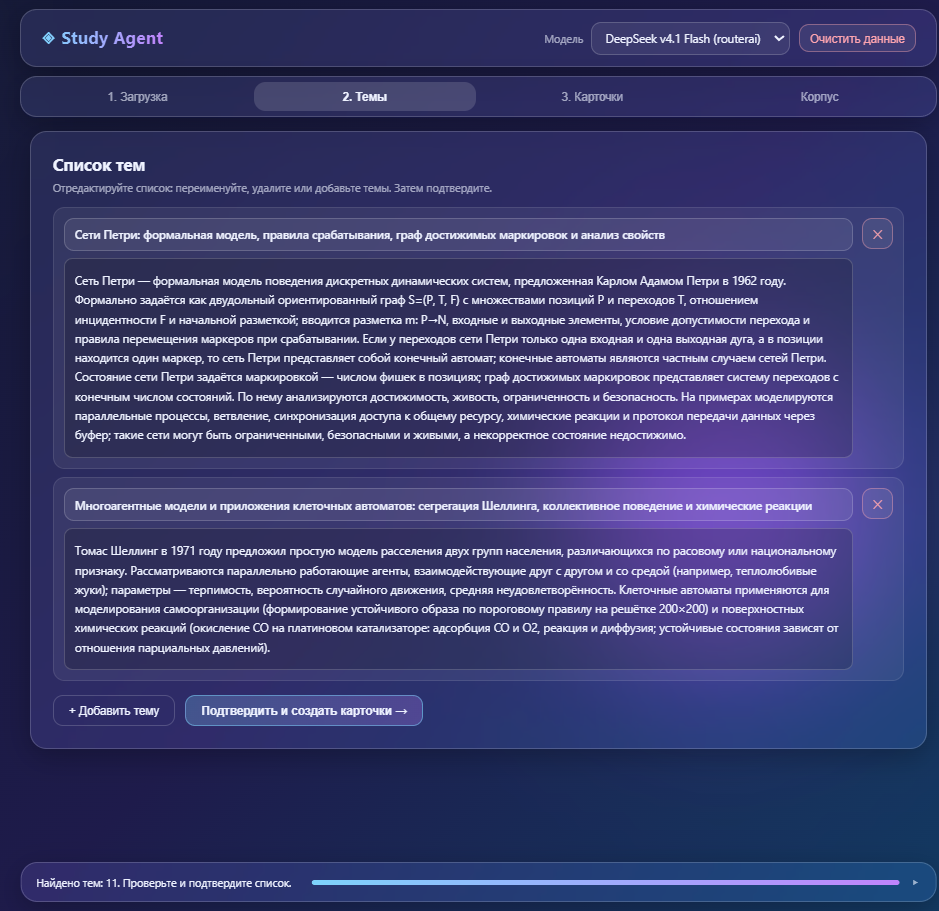
\includegraphics[width=0.85\textwidth]{images/темы.png}
    \caption{Список извлечённых тем для проверки и подтверждения}
    \label{fig:topics}
\end{figure}

Все этапы обработки отображаются в журнале событий в реальном времени
с указанием прогресса (рис.~\ref{fig:logs}).
\begin{figure}[H]
    \centering
    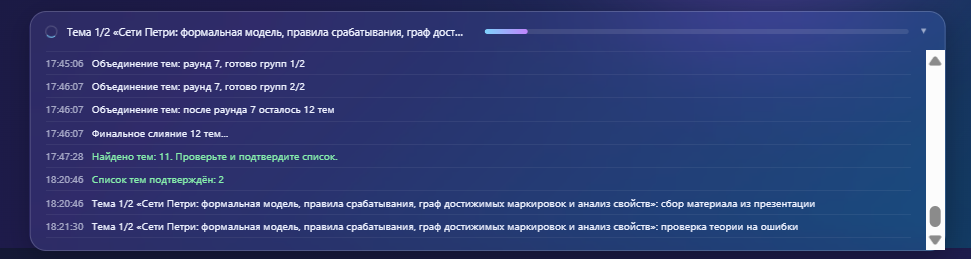
\includegraphics[width=0.85\textwidth]{images/логи.png}
    \caption{Журнал событий агента в реальном времени}
    \label{fig:logs}
\end{figure}

По завершении обработки формируются карточки тем с разделами <<Как в презентации>>,
<<Простым языком>>, <<Найденные ошибки в теории>> и <<Примеры из интернета>>,
а также полем для вопросов ИИ (рис.~\ref{fig:cards}).
\begin{figure}[H]
    \centering
    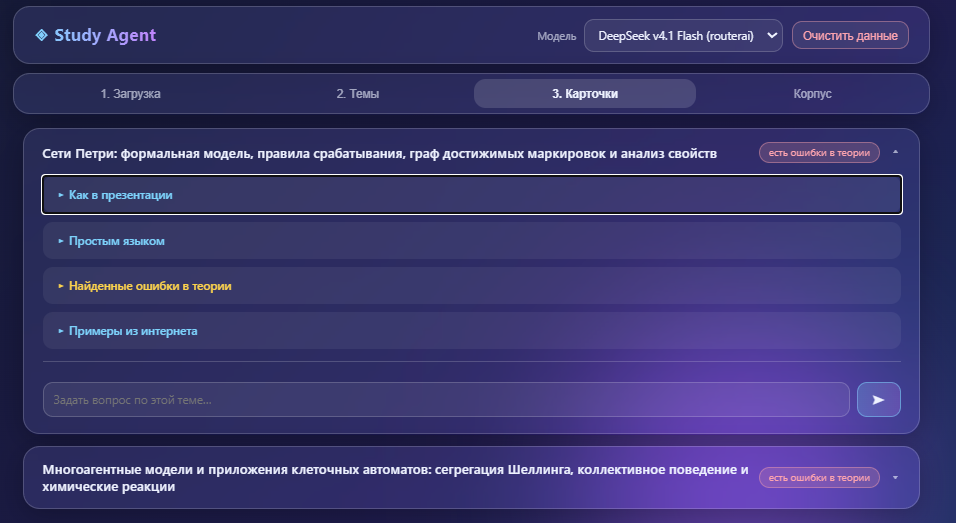
\includegraphics[width=0.85\textwidth]{images/карточки.png}
    \caption{Список сформированных карточек тем}
    \label{fig:cards}
\end{figure}

На рисунке~\ref{fig:card-detail} показана раскрытая карточка с разбором
найденной ошибки: агент приводит дословный фрагмент презентации, объясняет,
в чём состоит ошибка, и даёт правильную формулировку.
\begin{figure}[H]
    \centering
    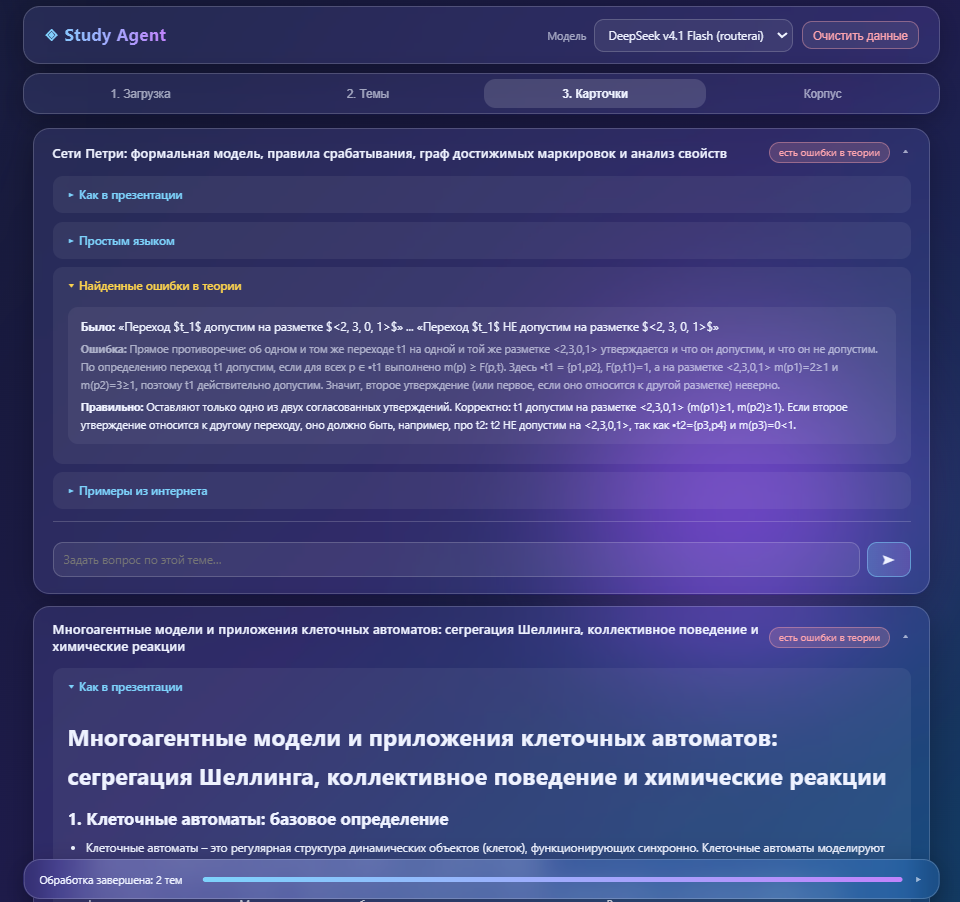
\includegraphics[width=0.85\textwidth]{images/карточки_подробнее.png}
    \caption{Карточка темы с разбором найденной в презентации ошибки}
    \label{fig:card-detail}
\end{figure}



